\documentclass[10pt,aspectratio=169]{beamer}

% All the boilerplate is in deslides.sty
\usepackage{deslides}

\author{Ji\v{r}\'i Lebl}

\institute[OSU]{%
Oklahoma State University%
%Departemento pri Matematiko de Oklahoma {\^S}tata Universitato%
}

\title{10. Numerical methods: Euler's method\\(Notes on Diffy Qs, 1.7)}

\date{}

\begin{document}

\begin{frame}
\titlepage

%\bigskip

\begin{center}
The textbook: \url{https://www.jirka.org/diffyqs/}
\end{center}
\end{frame}

\begin{frame}
It is often hard to find closed form solutions to
\quad
$y' = f(x,y)$, \quad $y(x_0) = y_0$.

\medskip
\pause

But we want answers!

\pause
Enter numerical methods:

Given a function $f(x,y)$ and numbers $x_0$, $y_0$, and $x_1$, get (approximately) $y(x_1)$.

\medskip
\pause

Not ideal, but sometimes best that we got.

\begin{itemize}
\item \pause
We need to know $f(x,y)$, $x_0$, $y_0$, $x_1$ exactly, we can't have parameters.
\item \pause
Hard to get qualitative understanding from a numerical solution.
\item \pause
It is only approximate, so we'd better understand the errors.
\item \pause
Must choose the right method.
\end{itemize}

\pause
\medskip

We will cover the simplest method of all: Euler's method.

\end{frame}

\begin{frame}

Euler's method for \quad
$y' = f(x,y)$, \quad $y(x_0) = y_0$.

\begin{enumerate}
\item
\pause
Pick a step size $h$.
\item
\pause
Compute the slope $k = f(x_0,y_0)$ at $(x_0,y_0)$.
\item
\pause
Follow the line of slope $k$ for $x$ from $x_0$ to $x_0+h$.
\item
\pause
That is, the new point $(x_1,y_1)$ is \quad
$x_1 = x_0+h$ \quad $y_1 = y_0 + h k$.
\item
\pause
Compute $k = f(x_1,y_1)$.
\item
\pause
Let $x_2 = x_1+h$ \quad $y_2 = y_1 + h k$.
\item
\pause
Compute $k = f(x_2,y_2)$.
\item
\pause
Let $x_3 = x_2+h$ \quad $y_3 = y_2 + h k$.
\item
\pause
Rinse, repeat!
\end{enumerate}

\pause
Essentially, keep repeating : \quad $x_{i+1} = x_i + h$, \quad $y_{i+1}  = y_i + h\, f(x_i,y_i)$.
\end{frame}

\begin{frame}
\textbf{Example:} \quad $y' = \nicefrac{y^2}{3}$, \quad $y(0)=1$, \quad $h=1$.

\medskip

\uncover<2-9>{
$x_0 = 0$, \quad $y_0 = 1$
}

\medskip

\uncover<3-9>{
$k = f(0,1) = \nicefrac{1^2}{3} = \nicefrac{1}{3}$
}

\uncover<4-9>{
$x_1 = x_0+h = 0+1 = 1$
}

\uncover<5-9>{
$y_1 = y_0 + h k = 1 + 1 \cdot
(\nicefrac{1}{3}) = \nicefrac{4}{3} \approx 1.333$
}

\medskip

\uncover<6-9>{
$k = f(1,\nicefrac{4}{3}) = \frac{(4/3)^2}{3} = \frac{16}{27}$
}

\uncover<7-9>{
$x_2 = x_1+h = 1+1 = 2$
}

\uncover<8-9>{
$y_2 = y_1 + h k = \nicefrac{4}{3} + 1 \cdot
(\nicefrac{16}{27}) = \nicefrac{52}{27} \approx 1.926$
}

\medskip

\vspace*{-1.6in}
\hspace*{\fill}%
\only<1>{\phantom{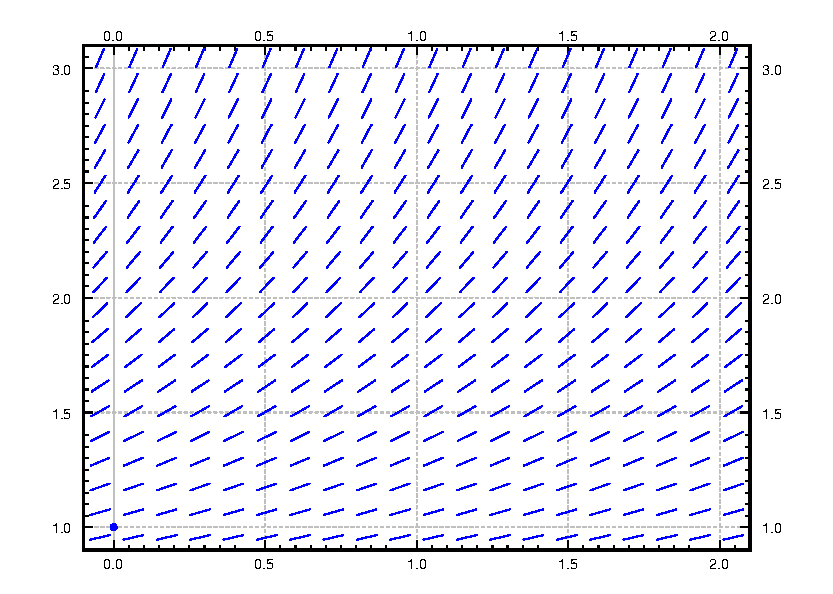
\includegraphics[width=2.8in]{figures/eulerexsl-0step}}}%
\only<2-4>{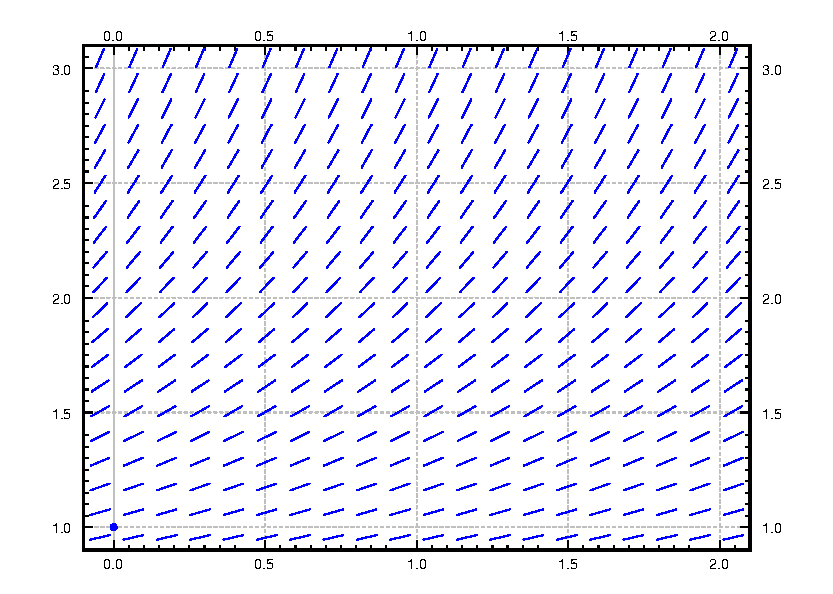
\includegraphics[width=2.8in]{figures/eulerexsl-0step}}%
\only<5-7>{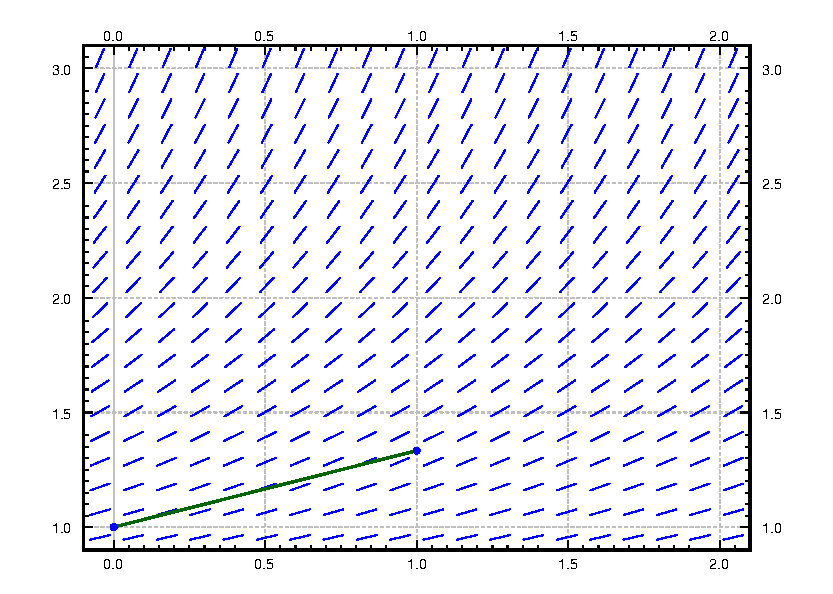
\includegraphics[width=2.8in]{figures/eulerexsl-1step}}%
\only<8>{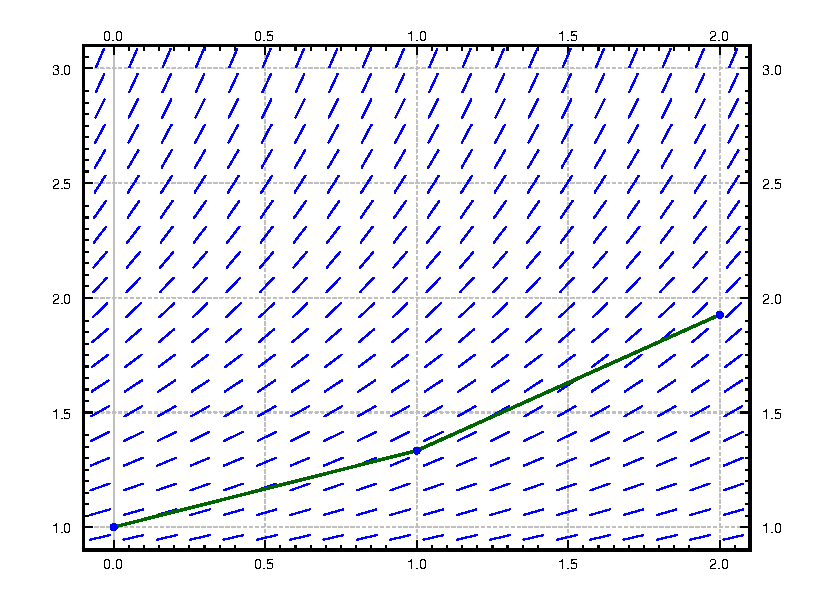
\includegraphics[width=2.8in]{figures/eulerexsl-2step}}%
\only<9>{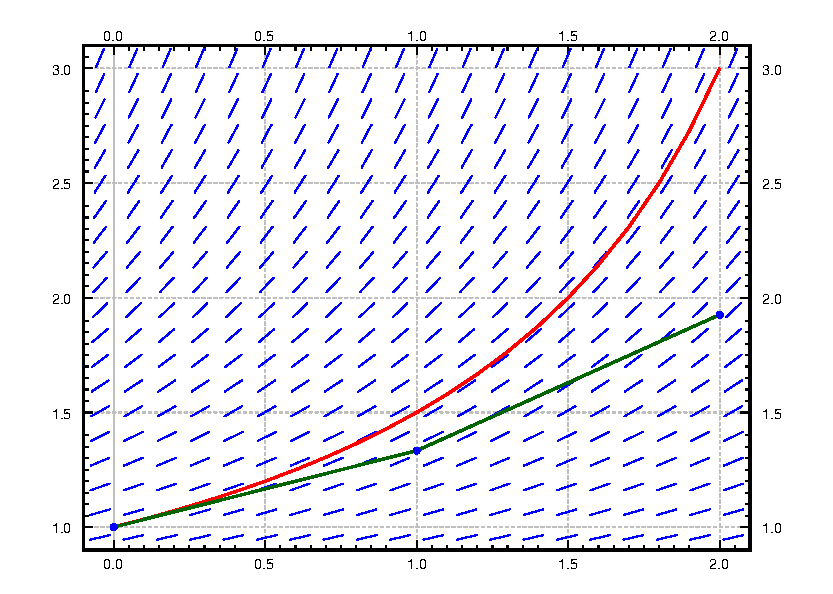
\includegraphics[width=2.8in]{figures/eulerexsl-2step-sol}}%

\end{frame}

\begin{frame}

Let's do a few more $h$s.

\bigskip

\hspace*{\fill}%
\only<1>{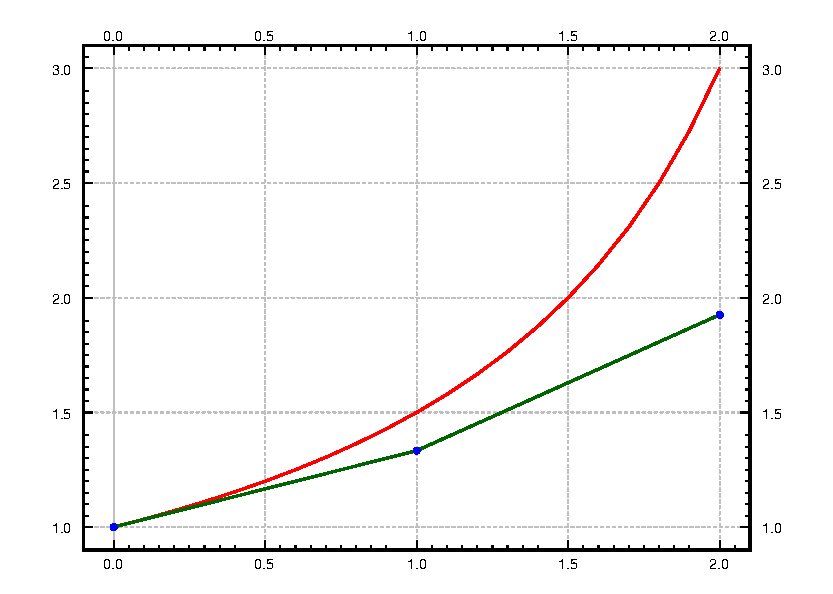
\includegraphics[width=3in]{figures/eulerex-h1}}%
\only<2>{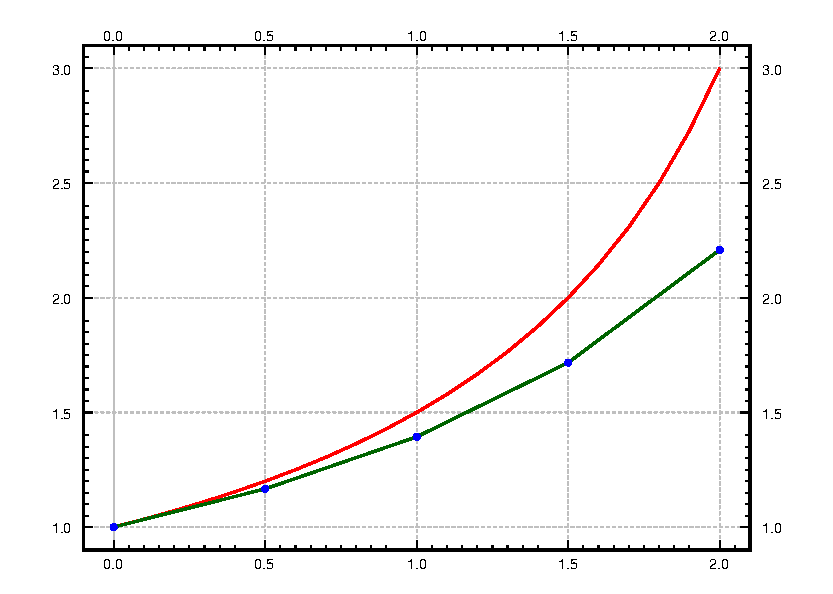
\includegraphics[width=3in]{figures/eulerex-h0.5}}%
\only<3>{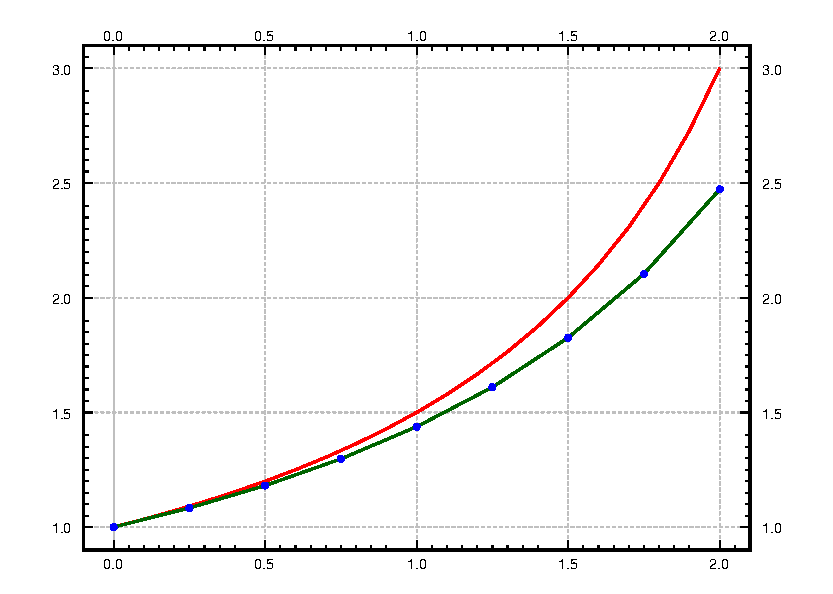
\includegraphics[width=3in]{figures/eulerex-h0.25}}%
\only<4>{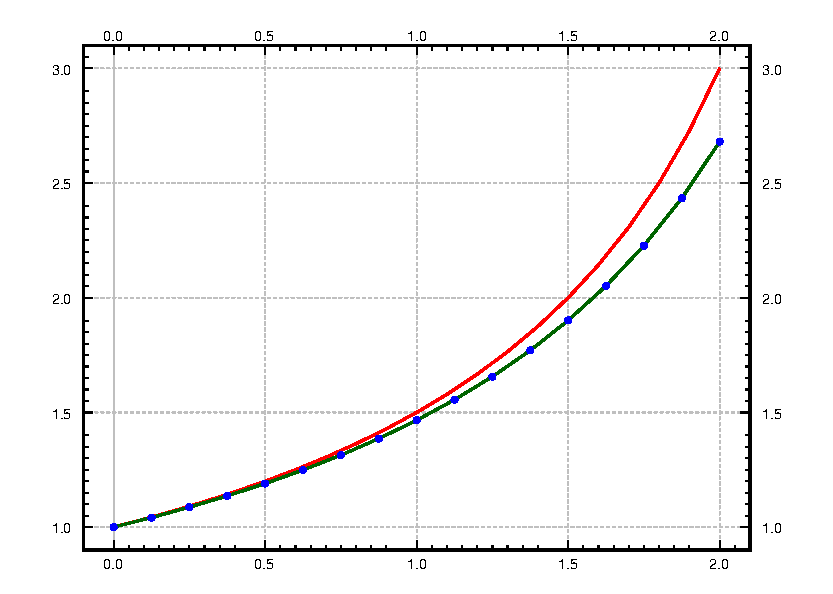
\includegraphics[width=3in]{figures/eulerex-h0.125}}%
\only<5>{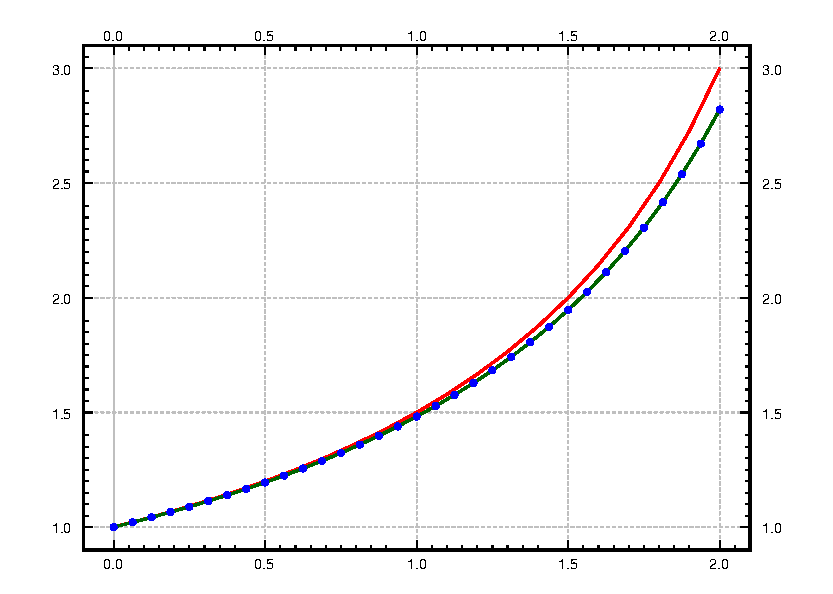
\includegraphics[width=3in]{figures/eulerex-h0.0625}}%
\only<6>{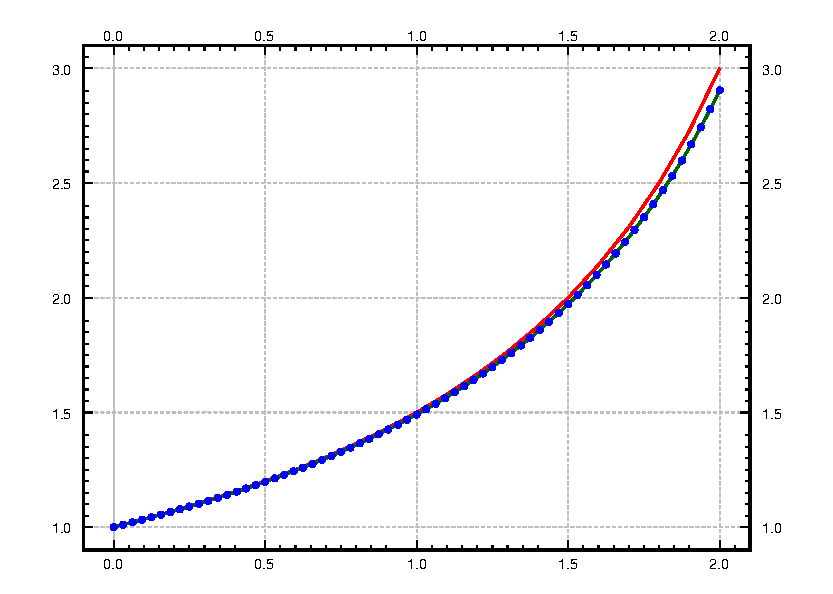
\includegraphics[width=3in]{figures/eulerex-h0.03125}}%
\hspace*{\fill}

\medskip

\only<1>{\begin{center}$h=1\vphantom{\nicefrac{1}{1}}$\end{center}}%
\only<2>{\begin{center}$h=\nicefrac{1}{2}=0.5$\end{center}}%
\only<3>{\begin{center}$h=\nicefrac{1}{4}=0.25$\end{center}}%
\only<4>{\begin{center}$h=\nicefrac{1}{8}=0.125$\end{center}}%
\only<5>{\begin{center}$h=\nicefrac{1}{16}=0.0625$\end{center}}%
\only<6>{\begin{center}$h=\nicefrac{1}{32}=0.03125$\end{center}}%
\end{frame}

\begin{frame}
Actual solution at $x=2$ is $y(2) = 3$.

\medskip
\pause

The absolute value of difference between the actual solution and the approximate solution is
called the \emph{error}.

\medskip
\pause

With $h=1$, $x_2=2$ so $y(2) \approx y_2 = 1.926$ 
\qquad
\pause
Error ${}=\lvert 3-y_2 \rvert \approx 1.074$

\medskip
\pause

With $h=\nicefrac{1}{2} = 0.5$, $x_4=2$ so $y(2) \approx y_4 = 2.209$
\qquad
\pause
Error ${}=\lvert 3-y_4 \rvert {}\approx 0.791$

\medskip
\pause

\hspace*{\fill}
\begin{tabular}{@{}rrrr@{}}
\toprule
$h$ & Approximate $y(2)$ & Error & $\frac{\text{Error}}{\text{Previous error}}$ \\
\midrule
1        & 1.92593 & 1.07407 & \\
0.5      & 2.20861 & 0.79139 & 0.73681 \\
0.25     & 2.47250 & 0.52751 & 0.66656 \\
0.125    & 2.68034 & 0.31966 & 0.60599 \\
0.0625   & 2.82040 & 0.17960 & 0.56184 \\
0.03125  & 2.90412 & 0.09588 & 0.53385 \\
0.015625 & 2.95035 & 0.04965 & 0.51779 \\
0.0078125& 2.97472 & 0.02528 & 0.50913 \\
\bottomrule
\end{tabular}
\hspace*{\fill}

\medskip
\pause

Note: It seems like error halves when we halve $h$.

\end{frame}

\begin{frame}

Euler's method is a \emph{first order method}:
When we halve $h$, error reduces by $\nicefrac{1}{2}$.

\medskip
\pause

A \emph{second order method} reduces the error by
$(\nicefrac{1}{2})^2 = \nicefrac{1}{4}$ each time you halve $h$.

\medskip
\pause

A \emph{fourth order method} reduces the error by
$(\nicefrac{1}{2})^4 = \nicefrac{1}{16}$ each time you halve $h$.

\medskip
\pause

To be within $0.1$ we needed to do 64 steps of Euler.

\medskip
\pause

To get within 0.01, we'd need another 2--3 halvings: so 512 to 1024 steps.

\medskip
\pause

If starting with one step, 10 halvings ${} = 2^{10} = 1024$ steps.

\medskip
\pause

A second order method requires half as many halvings for same
reduction of error.

\medskip
\pause

5 halvings ${} = 2^{5} = 32$ steps.

\medskip
\pause

That can be a huge difference if we need to run this many times.
\end{frame}

\begin{frame}
In practice we don't know the error, we must estimate it.

\medskip
\pause

By successive halvings, and assuming it halves each time we can estimate the
error.

\medskip
\pause

\textbf{Exercise:} Take the last two approximate values, and (assume they
are less than $y(2)$) assuming that the error halves each time, approximate
$y(2)$, and hence the error.  Is it close?

\medskip

\hspace*{\fill}
\begin{tabular}{@{}rrrr@{}}
\toprule
$h$ & Approximate $y(2)$ & Error & $\frac{\text{Error}}{\text{Previous error}}$ \\
\midrule
1        & 1.92593 & 1.07407 & \\
0.5      & 2.20861 & 0.79139 & 0.73681 \\
0.25     & 2.47250 & 0.52751 & 0.66656 \\
0.125    & 2.68034 & 0.31966 & 0.60599 \\
0.0625   & 2.82040 & 0.17960 & 0.56184 \\
0.03125  & 2.90412 & 0.09588 & 0.53385 \\
0.015625 & 2.95035 & 0.04965 & 0.51779 \\
0.0078125& 2.97472 & 0.02528 & 0.50913 \\
\bottomrule
\end{tabular}
\hspace*{\fill}

\medskip
\pause

The trick in practice is to estimate the error so that we can pick the right
$h$.

\end{frame}

\begin{frame}
Keep considering
\quad $y' = \nicefrac{y^2}{3}$, \quad $y(0) = 1$.

\medskip
\pause

Suppose we attempt to find $y(3)$:

\begin{center}
\begin{tabular}{@{}rr@{}}
\toprule
$h$ & Approximate $y(3)$ \\
\midrule
1        & 3.16232 \\
0.5      & 4.54329 \\
0.25     & 6.86079 \\
0.125    & 10.80321 \\
0.0625   & 17.59893 \\
0.03125  & 29.46004 \\
0.015625 & 50.40121 \\
0.0078125& 87.75769 \\
\bottomrule
\end{tabular}
\end{center}

\pause
What is going on? \pause $y(3)$ does not exist, \pause $y \to \infty$ as $x \to 3$.

\end{frame}

\begin{frame}

In real applications, methods used are similar to Euler
but better (e.g., the fourth order Runge--Kutta, see next slide).

\medskip
\pause

Choosing $h$ is very tricky.  A couple of things to consider:

\begin{itemize}
\item
\pause
Computational time: Each step takes computer time.
\item
\pause
Roundoff errors: Computers only compute with a certain number of
significant digits.
\item
\pause
Stability: Certain equations may be numerically unstable, sometimes
called \emph{stiff} problems.  Halvings may not seemingly improve things.
\end{itemize}

\medskip
\pause

In worst case, the computer might be giving us bogus numbers as if they are
correct.

\medskip
\pause

Numerical methods are still a current research topic.
\end{frame}

\begin{frame}

The simplest method used in practice is the
\emph{Runge--Kutta method}.

Consider $\frac{dy}{dx}=f(x,y)$, $y(x_0) = y_0$, and a step size $h$.

\medskip
\pause

The idea is the same as Euler except each step looks like
\begin{align*}
& k_1 = f(x_i,y_i) , & & \\
& k_2 = f\bigl(x_i + \nicefrac{h}{2},y_i + k_1 (\nicefrac{h}{2})\bigr) ,
& & 
x_{i+1} = x_i + h , \\
& k_3 = f\bigl(x_i + \nicefrac{h}{2},y_i + k_2 (\nicefrac{h}{2})\bigr) ,
& &
y_{i+1} = y_i + \frac{k_1 + 2k_2 + 2k_3 + k_4}{6}\,h ,  \\
& k_4 = f(x_i + h,y_i + k_3 h) .
\end{align*}

\end{frame}

\end{document}
